\documentclass{article}

\usepackage[utf8]{inputenc}
\usepackage{microtype}
\usepackage{listings}
\usepackage{tabularx}
\usepackage{url}
\usepackage{pgfplots}
\usepackage{mathtools}
\usepackage{csquotes}
\usepackage[center,width=.8\linewidth]{caption}

\pgfplotsset{compat=1.14}

\newcolumntype{R}{>{\raggedleft\arraybackslash}X}%

\title{CS3910 Computational Intelligence:\\Cutting Stock Problem (Coursework 1)}
\author{Scott Street\\{\small 159027651}}
\date{December 2017}

\begin{document}
\maketitle

\section{Introduction}

  The Cutting Stock Problem (CSP) is a combinatorial optimisation problem, in which we are given a set of stock lengths with associated costs, a set of order lengths with associated quantities, and must cut the ordered lengths from the given stock, while attempting to minimise the cost of materials.

  \bigskip

  For this coursework, implementations have been written in the Go programming language, for its high efficiency and concurrency features (not used in this version of the implementation, but potentially in future versions).

\section{Problem Representation}

  The problem instance is represented as a simple \lstinline{struct} containing the provided stock lengths, stock costs, order lengths, and order quantities. Each of these is contained within a \lstinline{slice} (variable length array).

  \bigskip

  Solutions to a problem instance are implemented as a 2D \lstinline{slice} of \lstinline{int}s, where the top level represents the available stock lengths, and the individual elements represent ordered lengths. It is not necessary to keep track of how many stock lengths of each type have been used, as it is not required for the running of either of the implemented algorithms, and can be calculated from this representation when needed.

\section{Algorithm Implementations}

  The Artificial Immune System (AIS) and Ant Colony Optimisation (ACO) algorithms were selected for use due to the combinatorial nature of the CSP. Both algorithms are well suited to such problems, whereas algorithms which are typically used to solve, for example, continuous problems are not as easily translated for use in this situation.

  \subsection{Artificial Immune System}

    The AIS approach is inspired by the human immune system. Specifically, the Clonal Selection algorithm (CLONALG) applies the theory that white blood cells improve their ability to counter alien cells over time, as they are exposed to them. In the case of the CSP, the algorithm improves its ability to produce more optimal solutions as it discovers them.

    \bigskip

    It does this through a method of cloning, mutation, and selection. From an initial population of a specified size, a clone pool is created by ``copying'' the existing population x-number of times (a parameter to the algorithm). The pool is then mutated through some process. In this implementation, the mutation function selects a random neighbour from the solution's two-opt neighbourhood.

    \bigskip

    The mutated pool is then added back to the main population, at which point the selection process takes place. This decides which of the population are kept for the next generation, up to a defined number. A simple greedy method of selection has been used in this instance.

    \bigskip

    Finally, a form of metadynamics are performed on the population - the lowest n-number of the populus are replaced by random solutions. Additionally, the ``age'' of each solution in the population is incremented, until reaching the defined maximum age, at which point is it removed from the population. Both of these methods prevent the algorithm from reaching ``stale'' solutions, or local minima. By ensuring this degree of randomness, we are guaranteed to eventually reach the optimal solution for a given problem instance.

  \subsection{Ant Colony Optimisation}

    The ACO algorithm is based on the behaviours of ants in a colony when trying to find an optimal route to a source of food. Individual ants deposit pheromones along the path they take, with shorter routes being travelled more frequently, thus greater pheromone deposition along these paths. This is an approach typically applied to ordering problems, for example the Travelling Salesperson Problem, due to the simple definition of pheromones in the algorithm as representing paths between nodes in a route. The pheromone trail definition is in fact a key component to producing desirable solutions, and is not immediately clear with the CSP.

    \bigskip

    In Ducatelle and Levine's \textit{Ant Colony Optimisation for Bin Packing and Cutting Stock Problems}\cite{acoforcsp}, it is suggested that pheremones should encode \enquote{the favourability of having an item of length \(i\) and length \(j\) in the same \textelp{} stock}. The ACO algorithm implemented here follows this suggestion, and additionally has taken other advice from the paper, such as good potential values for the weighting of the heuristic information compared with the pheromone for use in deciding the probability of a particular choice when constructing a solution.

    \bigskip

    Unfortunately, the results from my ACO implementation were not as good as I had hoped. It was in fact found to produce only marginally better results than a random search algorithm for the most part.

\section{Comparison of Algorithms}

  Based on initial runs of each algorithm on problem instances of different sizes, the AIS algorithm appeared to produce far more optimal solutions than the ACO algorithm, regardless of instance size. I was also unable to tweak the ACO algorithm parameters to produce solutions of cost significantly close to those of the AIS algorithm. Based on these observations, I constructed my hypotheses.

  \begin{table}[h]
    \begin{tabularx}{\textwidth}{ |l|R|R|R|R|R|R| }
      \hline
      \multicolumn{7}{|c|}{\textbf{CSP Problem 1 (Avg. over 40 runs)}} \\
      \hline
      Runs    & 1     & 5     & 10    & 20    & 40    & 80             \\
      \hline
      ACO     & 1586  & 1532  & 1482  & 1449  & 1409  & 1382           \\
      \hline
      CLONALG & 1409  & 1320  & 1295  & 1285  & 1283  & 1278           \\
      \hline
      Random  & 1603  & 1515  & 1478  & 1463  & 1453  & 1416           \\
      \hline
    \end{tabularx}
    \caption{Average results of different numbers of iterations over 40 algorithm runs on CSP instance 1.}
  \end{table}
  \begin{table}[h]
    \begin{tabularx}{\textwidth}{ |l|R|R|R|R|R|R| }
      \hline
      \multicolumn{7}{|c|}{\textbf{CSP Problem 2 (Avg. over 40 runs)}} \\
      \hline
      Runs    & 1     & 5     & 10    & 20    & 40    & 80             \\
      \hline
      ACO     & 5533  & 5446  & 5428  & 5362  & 5278  & -              \\
      \hline
      CLONALG & 5175  & 5044  & 4926  & 4804  & 4660  & 4542           \\
      \hline
      Random  & -     & -     & -     & -     & -     & -              \\
      \hline
    \end{tabularx}
    \caption{Average results of different numbers of iterations over 40 algorithm runs on CSP instance 2.}
  \end{table}

  I formulated my null hypothesis that the AIS algorithm is, on average, no better than the ACO algorithm at solving problem 3 (\textit{cutting\_problem\_instance.txt}) in terms of lowest cost solution found after 1000 iterations. My alternate hypothesis was that the AIS algorithm is, on average, \textit{better} than the ACO algorithm at solving problem 3 in terms of lowest cost solution found after 1000 iterations.

  \bigskip

  To test these hypotheses I ran both algorithms for 1000 iterations, 40 times each, and took a mean average of the results. This was sufficient to be used as a representative average of both algorithms. On comparison, the mean of the AIS algorithm (2058) was significantly lower than that of the ACO algorithm (2212), implying that it will likely be possible to reject the null hypothesis. Applying Welch's t-test to the dataset, an \(\alpha\) value very close to zero was returned, lower than the significance level of \(\alpha = 0.05\), allowing me to reject the null hypothesis and claim that the AIS algorithm is in fact on average better than the ACO algorithm at solving problem 3 in terms of lowest cost solution found after 1000 iterations.

  \begin{figure}[h]
    \begin{center}
      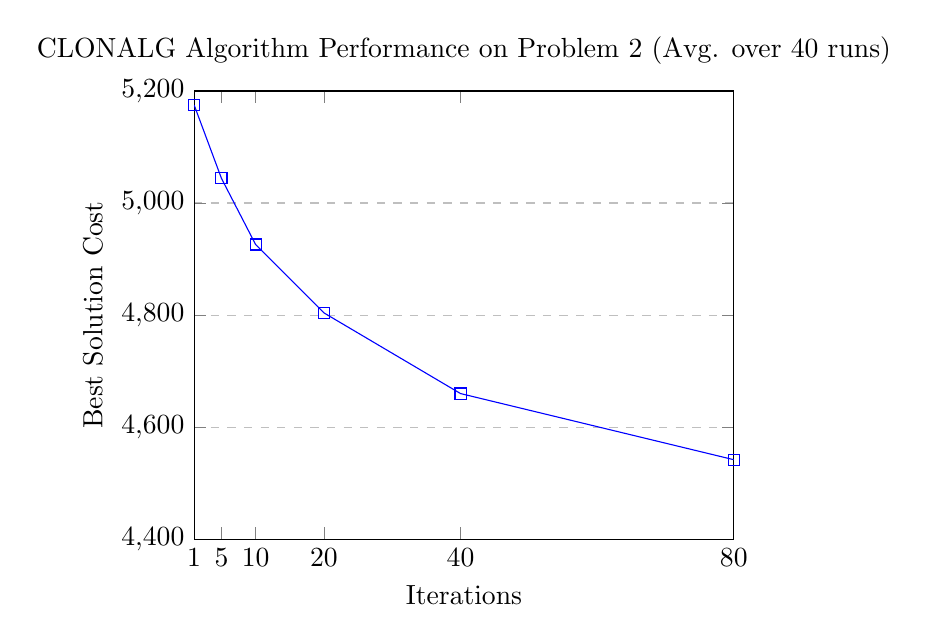
\begin{tikzpicture}
        \begin{axis}[
            title={CLONALG Algorithm Performance on Problem 2 (Avg. over 40 runs)},
            xlabel={Iterations},
            ylabel={Best Solution Cost},
            xmin=1, xmax=80,
            ymin=4400, ymax=5200,
            xtick={1,5,10,20,40,80},
            ytick={4400,4600,4800,5000,5200},
            legend pos=north west,
            ymajorgrids=true,
            grid style=dashed,
        ]

          \addplot[
              color=blue,
              mark=square,
              ]
              coordinates {
              (1,5175)(5,5044)(10,4926)(20,4804)(40,4660)(80,4542)
              };

        \end{axis}
      \end{tikzpicture}
    \end{center}
  \end{figure}

  \bigskip

\bibliography{report}
\bibliographystyle{plain}

\end{document}
